%!TEX root = ../thesis.tex
%*******************************************************************************
%*********************************** First Chapter *****************************
%*******************************************************************************

\chapter{Introduction}

\ifpdf
    \graphicspath{{Chapter1/Figs/Raster/}{Chapter1/Figs/PDF/}{Chapter1/Figs/}}
\else
    \graphicspath{{Chapter1/Figs/Vector/}{Chapter1/Figs/}}
\fi


%********************************** %First Section  **************************************
\section{From background to foreground}

Radio astronomers Arno Penzias and Robert Wilson were calibrating their 50-feet-long horn antenna when they found a mysterious background noise. The measurements were independent of time and location in the sky, and persisted after the removal of various potential contaminants. After the theoretical work of Robert Dicke, Jim Peebles, and David Wilkinson was brought forward \cite{Dicke1965}, Penzias and Wilson identified the noise as cosmic microwave background radiation (CMB): ancient light from the early universe reaching us after billions of years \cite{Penzias1965}. The discovery provided us with one of the most valuable probes of the physical universe, leading to major development in observational cosmology.

On the theoretical side, modern mathematical formulation of cosmology owes to Einstein's work on general relativity in 1915. Using his framework, Friedmann, Lemaître, Robertson, and Walker contributed to writing down the unique metric for spatially homogeneous and isotropic universe. The FLRW metric dictates growth of the universe from the Big Bang to present day. Such expansion of the universe was supported by Edwin Hubble's measurements of Cepheid variables and redshift (add year), as well as the aforementioned discovery of CMB. What is widely accepted to be the standard model of modern cosmology, the $\Lambda$CDM model, appeared only in the late 1990s. The six-parameter model assumes presence of cold dark matter and dark energy, in addition to baryons and radiation, as main contributors to the total energy density of the universe.

The $\Lambda$CDM model has been extremely successful in explaining modern cosmological observations. CMB measurements from \textit{Planck} satellite, in particular, show exceptional agreement with the model. Planck was a space observatory developed by the European Space Agency. The Planck satellite observed the CMB in nine frequency bands from 2009 to 2013, with resolution and sensitivity substantially improved compared to its predecessor - the Wilkinson Microwave Anisotropy Probe (WMAP). Able to resolve CMB anisotropy in much smaller scale, Planck placed one of the most stringent bounds on the theoretical parameters of $\Lambda$CDM so far.

How does CMB contain so much information about the universe? The answer is twofold. First is due to the fact that CMB anisotropy originates from primordial perturbations. Statistical properties of the initial fluctuations can be deduced from analysing correlation functions of the CMB, letting us constrain the early universe physics. Second reason is that CMB tracks history of the universe as it travels from the background to our foreground. CMB photons scatter with baryons before free-streaming all the way to our foreground, which then experience both growth of the universe and gravitational potential of matter perturbations. These signatures are engraved in CMB anisotropy spectrum, redshift, and weak lensing.

The CMB anisotropy is observed to be nearly Gaussian distributed. Statistical characteristics of a Gaussian random field can be summarised entirely using two-point correlation functions, or their Fourier counterpart: power spectrum. The CMB power spectra have been thoroughly studied to constrain various cosmological parameters. Meanwhile, higher-order statistics such as three-point correlation functions (bispectrum in Fourier space) also contain valuable information about our universe. They probe non-Gaussian statistics of the CMB arising from both primordial origin and late-time effects.

Primordial non-Gaussianity is a key statistic for studying physics of the early universe. The theory of inflation has been successful in describing the observed data, but its exact mechanism is yet undetermined. Currently there are numerous viable inflationary models with well-founded physical motivations. Non-Gaussian signatures of primordial fluctuations are robust predictions of various models, and measuring their shape and amplitude allows us to constrain inflationary scenario. CMB bispectrum analysis from Planck yielded the most precise measurements of primordial non-Gaussianity to date. So far, no statistically significant amount of non-Gaussianity has been detected.

In the near future, we expect several new major CMB experiments. Simons Observatory (SO) is a ground-based experiment currently under construction in the Atacama Desert of Chile. SO is expected to measure both CMB temperature and polarisation to unprecedented precision, largely improved compared to Planck. The first light from SO is planned to be observed in early 2022. Many more CMB Stage-4 (CMB-S4) experiments are proposed, brightening future prospects for CMB. In particular, the upcoming measurements will allow us to constrain primordial non-Gaussianity further, providing discovery potential.

This thesis is organised as follows. In Chapter 1, we review the standard formulation of cosmology, deriving the form of scale factor in homogeneous universe. Motivation and formalism of slow-roll inflation is also presented here. Chapter 2 details cosmological perturbation theory, with a focus on the CMB anisotropy. We summarise methods for computing the transfer function of CMB, and introduce the concept of CMB polarisation. Next, in Chapter 3 we define bispectrum and discuss how it can be used to probe primordial non-Gaussianity. An example of single-field inflation with non-canonical kinetic term will be provided to demonstrate computation of non-Gaussianity using the in-in formalism.

Chapter 4 and 5 contain my original work, based on research conducted in collaboration with my supervisor James Fergusson. Chapter 4 contains the forecast for future CMB-S4 surveys on the primordial non-Gaussianity parameter $f_{NL}$. SO experiment specifications and expected CMB-S4 setup were used to predict their improved constraints via Fisher information analysis. We focussed on models with oscillatory features, where steep enhancement in polarisation sensitivity greatly benefit constraining power.

Motivated by the positive prospects from forecasts detailed in Chapter 4, we worked on developing a high-resolution bispectrum estimation pipeline suitable for future surveys. Chapter 5 contains formulation and development details of the developed program, as well as consistency checks from the thorough verification process. We outline the benefits of new pipeline compared to conventional methods, and present some working examples. Lastly, Chapter 6 concludes the thesis by summarising and presenting plans for future research.

\section{The homogeneous universe}

In this section we review the standard cosmological formulation for the homogeneous universe, neglecting any perturbations. What we derive here will serve as a background solution for the full perturbative result discussed in the next chapter. We assume general relativity to be an accurate theory of gravity for relevant scales.

\subsection{Geometry}

In general relativity, spacetime is represented by a 4-dimensional Lorentzian manifold equipped with a metric. Distance measure in curved spacetime is given by the metric tensor $g$;
\begin{align}
	ds^2 \,=\, g_{\mu \nu} \; dx^\mu dx^\nu	,
\end{align}
where the Greek letters $\mu, \nu = 0,1,2,3$ represent time ($0$) and spatial ($1,2,3$) indices of local coordinates. Flat spacetime has metric $g_{\mu\nu} = \eta_{\mu\nu} = \text{diag}\{-1, 1, 1, 1\}$, also known as the Minkowski metric. Throughout this thesis we adopt the sign convention $(-, +, +, +)$ and work in units where $c=1$. Unless specified otherwise, the Einstein summation convention is assumed. 

In curved spacetime, free particles follow a trajectory given by the geodesic equation;
\begin{align}
	\frac{d^2x^\mu}{ds^2} \,+\, \Gamma^\mu_{\nu \rho} \frac{dx^\nu}{ds} \frac{dx^\rho}{ds} \,=\, 0,  \label{eqn:geodesic}
\end{align}
with $s$ an affine parameter parametrising the trajectory, and $\Gamma^\mu_{\nu\rho}$ the Christoffel symbol representing metric connection. Its value is given in terms of the metric tensor by
\begin{align}
	\Gamma^{\mu}_{\nu\rho} \,=\, \frac{1}{2}~ g^{\mu\sigma} \left( \partial_\rho g_{\nu\sigma} \,+\, \partial_\nu g_{\rho\sigma} \,-\, \partial_\sigma g_{\nu\rho}  \right). \label{def:Levi_Civita}
\end{align}
Here and throughout this thesis, $\partial_\mu$ denote the partial derivative with respect to local coordinate $x^\mu$. Note $g^{\nu\sigma}$ is the inverse metric satisfying $g^{\mu\nu} g_{\nu\rho} \,=\, \delta^\nu_\rho$.

Defining tangent vector as $U^\mu = dx^\mu / ds$, the equation can be rewritten in a covariant form given by
\begin{align}
	\left( \nabla_U U \right)^a \,=\, U^b \nabla_U U^a \,=\, 0.
\end{align}
We follow the convention where Roman letters are used for abstract indices. Note that in terms of local coordinates, the covariant derivative of a vector field is defined as $\nabla_\nu U^\mu = \partial_\nu U^\mu + \Gamma^\mu_{\nu\rho} U^\rho$.

Distance between two geodesics that are initially parallel may change in curved spacetime. Such geometric information is encapsulated within the Riemann curvature tensor $R^a_{bcd}$. \footnote{Consider a 1-parameter family of geodesics $\gamma(s,t)$, where $t$ is an affine parameter. The geodesic deviation equation states $T^\rho \nabla_\rho ( T^\nu \nabla_\nu S^\mu ) = R^\mu_{\nu\rho\sigma} T^\nu T^\rho S^\sigma$, where tangent vectors $T=\partial/\partial t$, $S=\partial/\partial s$.} From $R^a_{bcd}$ we can evaluate the Ricci curvature tensor $R_{ab}$, the Ricci scalar $R$, and finally the Einstein tensor $G_{ab}$. They are defined as follows.
\begin{align}
	R^\mu_{\nu\rho\sigma} \,:=& \,\, \partial_\rho \Gamma^\mu_{\nu\sigma} \,-\, \partial_\sigma \Gamma^\mu_{\nu\rho} \,+\, \Gamma^\tau_{\nu\sigma} \Gamma^\mu_{\tau\rho} \,-\, \Gamma^\tau_{\nu\rho} \Gamma^\mu_{\tau\sigma}  \label{def:Riemann_tensor}\\
	R_{\mu\nu} \,:=& \,\, R^\rho_{\mu\rho\nu}  \\ % Extra detail: \,=\, \partial_\rho \Gamma^\rho_{\mu\nu} \,-\, \partial_\nu \Gamma^\rho_{\mu\rho} \,+\, \Gamma^\tau_{\mu\nu} \Gamma^\rho_{\tau\rho} \,-\, \Gamma^\tau_{\mu\rho} \Gamma^\rho_{\tau\nu}
	R \,:=& \,\, g^{\mu\nu} R_{\mu\nu} \\
	G_{\mu\nu} \,:=& \,\, R_{\mu\nu} - \frac{1}{2} g_{\mu\nu} R \label{def:Einstein_tensor}
\end{align}

The Einstein tensor is symmetric, i.e. $G_{\mu\nu} = G_{\nu\mu}$. It is also important to note that its divergence vanishes; $\nabla^\mu G_{\mu\nu} = 0$, which can be proven using the contracted Bianchi identity.


\subsection{The FLRW universe}
On very large scales, our universe is observed to be uniform in space (homogeneous) and not have a favoured direction (isotropic). Spatial part of the homogeneous and isotropic metric has constant curvature and can be categorised into three: spherical ($\mathbb{S}^3$), Euclidean ($\mathbb{E}^3$), and hyperbolic ($\mathbb{H}^3$). They are induced from embedding $\mathbb{R}^3$ into submanifolds of $\mathbb{R}^4$ equipped with the Euclidean metric, defined as $K|\mathbf{x}|^2 + u^2 = 1$. Here $K=1,0,-1$ for $\mathbb{S}^3$, $\mathbb{E}^3$, and $\mathbb{H}^3$, respectively. Writing the embedding as $f: x^i = (x,y,z) \mapsto X^I =(x,y,z,\sqrt{1-K(x^2+y^2+z^2)})$, the induced metric
\begin{align}
	\gamma_{ij} := \frac{\partial X^I}{\partial x^i} \frac{\partial X^J}{\partial x^j} \delta_{IJ}
	= \delta_{ij} + \frac{x_i x_j}{1-Kx_k x^k}. \label{eqn:FLRW_metric_spatial}
\end{align}
The spatial line element is therefore given by
\begin{align}
	dl^2 = \gamma_{ij} dx^i dx^j =& d\mathbf{x} \cdot d\mathbf{x} + \frac{K(\mathbf{x} \cdot d\mathbf{x})^2}{1-K (\mathbf{x} \cdot \mathbf{x})} \\
	=& \frac{1}{1-Kr^2} dr^2 + r^2 d\Omega^2,
\end{align}
where the angular line element $d\Omega^2 = d\theta^2 + \sin^2\theta d\phi^2$.

We may now write down the form of the metric describing our universe in large scales;
\begin{align}
	ds^2 = - dt^2 + a(t)^2 \left( \frac{1}{1-Kr^2} dr^2 + r^2 d\Omega^2 \right).
\end{align}
This is known as the FLRW metric, named after independent researchers who worked on the topic. Function $a(t)$ is called the scale factor and it dictates the growth of universe over time. Note that the metric is invariant under rescaling $a \rightarrow \lambda a$, $r \rightarrow r / \lambda$, and $K \rightarrow k:= \lambda^2 K$. Hence we may set the scale factor to be $a(t_0) = 1$ at present time, at the cost of replacing $K \in \{-1,0,1\}$ by $k \in \mathbb{R}$.

Levi-Civita connection corresponding to the FLRW metric can be computed using the definition (\ref{def:Levi_Civita}). Its non-zero components are given as follows.
\begin{align}
	\Gamma^0_{ij} =& \frac{\dot{a}}{a} \gamma_{ij}, \\
	\Gamma^i_{j0} =& \Gamma^i_{0j} = \frac{\dot{a}}{a} \delta^i_j, \\
	\Gamma^i_{jk} =& \frac{1}{2a^2} \gamma^{il} \left( \partial_k \gamma_{jl} + \partial_j \gamma_{kl} - \partial_l \gamma_{jk} \right). 
\end{align}
Overdot denotes time derivative $(\,\, \dot{} \,\,) := \partial/\partial t$ here and for the rest of this thesis. Indices for $\gamma$ are raised and lowered using $\gamma$, not $g$.

Note that a path defined by $t(\tau)=\tau$ and $\mathbf{x}(\tau)=const$ is a timelike geodesic satisfying the geodesic equations (\ref{eqn:geodesic}). \textit{Comoving} observers who follow these paths continue to perceive the expanding universe to be isotropic. Meanwhile, they find themselves drift apart, as the physical distance $r_{phys} = a(t) r$ grows in time.

Ricci curvature and Einstein tensor of the FLRW metric follows from definitions (\ref{def:Riemann_tensor}-\ref{def:Einstein_tensor});
\begin{align}
	R_{00} =& - \frac{\ddot{3a}}{a} \\
	R_{ij} =& \left[ \frac{\ddot{a}}{a} + 2 \left( \frac{\dot{a}}{a} \right)^2 + \frac{2k}{a^2} \right] a^2 \gamma_{ij}, \label{eqn:FLRW_Ricci_spatial}\\
	R =& 6 \left[ \frac{\ddot{a}}{a} + \left( \frac{\dot{a}}{a} \right)^2 + \frac{k}{a^2} \right], \\
	G_{00} =& 3 \left[ \left( \frac{\dot{a}}{a} \right)^2 + \frac{k}{a^2} \right], \\
	G_{ij} =& \left[ - \frac{2\ddot{a}}{a} - \left( \frac{\dot{a}}{a} \right)^2 - \frac{k}{a^2} \right] a^2 \gamma_{ij}.
\end{align}
While deriving (\ref{eqn:FLRW_Ricci_spatial}) we used the fact that the Ricci tensor of three-dimensional spatial metric $\gamma$ is equal to $2k\gamma_{ij}$. \footnote{In general, the Ricci tensor of any $n$-dimensional constant-curvature space with metric $g_{ij}$ is given by $R_{ij} = (n-1)\kappa g_{ij}$. Here $\kappa$ denotes sectional curvature of the space, which is equal to $k$ for $\gamma$ defined in (\ref{eqn:FLRW_metric_spatial}).} Also note that components $G_{0i}$ vanish and $G_{ij} \propto g_{ij}$, which is expected for a spatially homogeneous and isotropic spacetime.

\subsection{Cosmic inventory}

According to general relativity, spacetime is curved by its contents. Objects interact with gravity through the energy-momentum tensor $T_{\mu\nu}$, which encapsulates their energy, momentum flux, and stress. Here, we assume that components of the homogenous universe can be modelled as \textit{perfect} fluids; they are completely characterised by rest frame energy density and isotropic pressure. Defining the 4-velocity to be $U^\mu = dx^\mu / ds$, the energy-momentum tensor of a perfect fluid is given by
\begin{align}
	T_{\mu\nu} = (\rho + P) U_\mu U_\nu + P g_{\mu\nu},
\end{align}
where the energy density $\rho$ and pressure $P$ only depends on time.

Note that the 4-velocity of From the geodesic equation (\ref{eqn:geodesic}), 

We further assume that components of the universe follow a simple equation of state $P = \omega \rho$. 

The universe consists of many different components, but they can be broadly categorised into three: radiation, matter, and dark energy. Radiation includes  Here, we assume that they are perfect fluids characterised by 


Cosmic inventory. Radiation, matter, dark energy. 

Divergence-free T -> conservation equations. Friedmann equations.

Critical density. $\Omega_X := \rho_X / \rho_{crit,0}$. Dependence on $a$. Radiation, Matter, Dark Energy domination.

Table of cosmic inventory. Type / Examples / Equation of state / $a$ dependence

Conformal time, growth of the universe.

Redshift


\begin{table}[h]
	\caption{Cosmic inventory. The fractional density values are quoted from CMB analysis (quote Planck 2018)}
	\centering
	\label{table:cosmic_inventory}
	\renewcommand{\arraystretch}{1.5} 
	\begin{tabular}{c | c | c | c | c}
		& Examples & Equation of State & Density Growth & Density Today \\ 
		
		\hline
		\multirow{2}{*}{Radiation $(r)$} & Photon $(\gamma)$ & \multirow{2}{*}{$\omega = 1/3$} & \multirow{2}{*}{$\rho \propto a^{-4}$} & $\Omega_{\gamma} \approx 1 \times 10^{-4}$ \\
		& Neutrino $(\nu)$ & & & $\Omega_{\nu} < 2 \times 10^{-2}$ \\

		\hline		
		\multirow{2}{*}{Matter $(m)$} & Cold dark matter $(c)$ & \multirow{2}{*}{$\omega = 0$} & \multirow{2}{*}{$\rho \propto a^{-3}$} & $\Omega_{c} \approx 0.27$ \\
		& Baryon $(b)$ & & & $\Omega_{b} \approx 0.05$ \\
		
		\hline
		Dark Energy $(\Lambda)$ & & $\omega=-1$ & $\rho=\text{const}$  & $\Omega_\Lambda \approx 0.68$\\
		\hline 
	\end{tabular}
\end{table}

\begin{table}[h]
	\caption{Evolution of the universe.}
	\centering
	\label{table:evolution_of_the_universe}
	\renewcommand{\arraystretch}{1.5} 
	\begin{tabular}{c | c | c | c | c}
		Era & Scale Factor & Growth (comoving) & Growth (conformal) \\ 
		
		\hline
		Radiation Domination (RD) & $a < 2.9 \times 10^{-4}$ & $a \propto t^{1/2}$ & $a \propto \tau$ \\
		\hline
		Matter Domination (MD) & $ 2.9 \times 10^{-4} < a < 0.77 $ & $a \propto t^{2/3}$ & $a \propto \tau^2$ \\
		\hline
		Dark Energy Domination ($\Lambda$D) & $a > 0.77$ & $a \propto e^{Ht}$ & $a \propto -1/\tau$ \\
		
		\hline 
	\end{tabular}
\end{table}

\section{Inflation}

\subsection{The horizon problem}

\begin{figure}[htbp!] 
	\centering    
	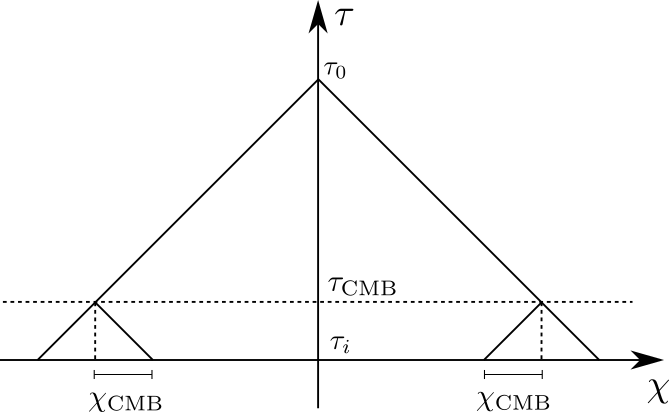
\includegraphics[width=0.7\textwidth]{horizon_problem.png}
	\caption[Horizon problem]{Horizon problem.}
	\label{fig:horizon_problem}
\end{figure}

\begin{figure}[htbp!] 
	\centering    
	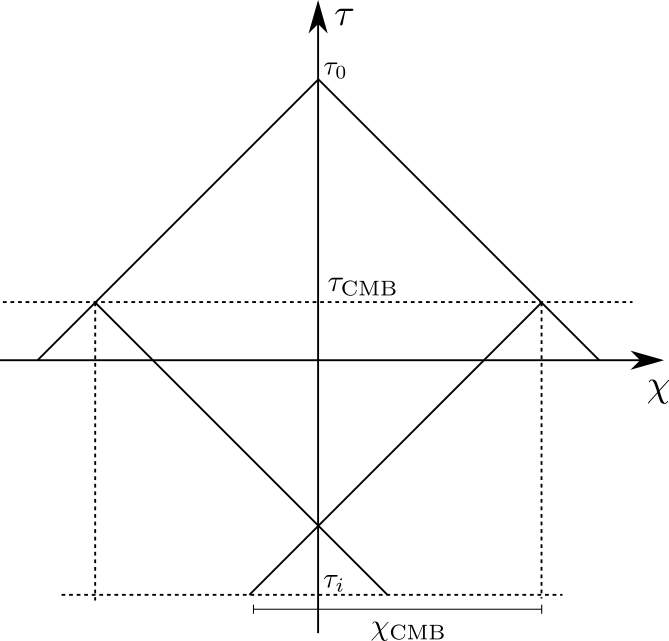
\includegraphics[width=0.7\textwidth]{horizon_solution.png}
	\caption[Horizon problem]{Solution to the horizon problem.}
	\label{fig:horizon_solution}
\end{figure}

\subsection{Slow-roll inflation}
